\chapter{Estado da Arte}

Neste capítulo é apresentado o estado da arte relativo ao contexto desta dissertação. 

\section{Introdução ao problema}

A plataforma \gls{clav} pode ser divididas em 3 eixos principais:

\begin{enumerate}
    \item \textbf{Frontend}
    Responsável pela interação dos utilizadores com plataforma, bem como chamadas à \gls{api}, podendo esta ser de cariz público ou privado, através do acesso a certas funcionalidades da plataforma (por exemplo: listagens de utilizadores, entidades, legislações, etc).
    
    \item \textbf{Backend}
    Desenvolvido em \emph{NodeJS}, este é responsável por satisfazer os serviços requisitados pelo \emph{Frontend}. Inclui toda a lógica da aplicação, como a camada de acesso a dados, leitura e armazenamento de informação.
    
    \item \textbf{API de dados}
    Responsável pela comunicação e gestão de pedidos dos utilizadores da plataforma, sendo que a sua principal função é servir de elo de ligação entre os resultados guardados em base de dados e o \emph{Frontend} disponibilizado aos utilizadores.
\end{enumerate}

Devido à natureza dos dados presentes na plataforma \gls{clav}, foi necessário proceder a uma correta e estruturada implementação de diversos mecanismos de segurança e proteção contra uso indevido de dados.

\cleardoublepage
\section{Soluções adoptadas}

De modo a oferecer um nível de segurança adequado à plataforma, foram adotadas várias medidas de segurança, sendo estas explicadas em mais detalhe nas subsecções seguintes.

\subsection{Gestão de utilizadores via Passport}

A gestão de utilizadores é feita através da combinação entre o middleware\footnote{Middleware é um software que funciona como intermediário entre dois programas.} designado por \emph{Passport} e a base de dados não-relacional\footnote{Estilo de base de dados livres de esquema, capazes de maior escalabilidade que as base de dados tradiconais.} implementada em \emph{MongoDB}.

Devido à informação sensível que pode ser guardada na mesma, campos como a password são, naturalmente, encriptados recorrendo a técnicas discutidas posteriormente.

%\subsubsection{Passport}
O \emph{Passport} é um middleware de autenticação, desenvolvido para \emph{NodeJS}, com mais de 500 estratégias\footnote{Uma estratégia pode ser interpretado como um mecanismo único de autenticação.} diferentes de autenticação. Foi criado para solucionar um único problema: \textbf{autenticar pedidos}.

Devido à natureza do \emph{Passport}, este é extremamente fácil de implementar numa dada aplicação, devido ao seu forte encapsulamento e ao facto de delegar qualquer funcionalidade, que não seja a autenticação, para a aplicação.

Devido à natureza das aplicações Web modernas, a autenticação pode ser feita por diversas estratégias. A estratégia utilizada neste projeto recaiu sobre a escolha mais "tradicional", uma autenticação local com campos para \emph{username} e \emph{password}.

Embora com o aumento exponencial da popularidade de implementações de autenticação baseadas em redes sociais, através de protocolos baseados em \emph{OAuth}\footnote{Protocolo open-source que permite autenticação de forma standard e segura, entre aplicações desktop, web e mobile.}, tais como \emph{Google+} e \emph{Facebook}, foi decidido desde uma fase inicial que tais estratégias não seriam consideradas devido ao carácter profissional da plataforma.

Devido a cada aplicação possuir necessidades diferentes, o \emph{Passport} guarda cada estratégia de autenticação em módulos independentes, deixando assim a cargo do programador que estratégias empregar, sem criar dependências desnecessárias.

De seguida será apresentada a forma como as passwords dos utilizadores estão a ser protegidas.

\cleardoublepage
\subsubsection{Encriptação de dados}

Em qualquer aplicação no mundo real, é impensável guardar dados sensíveis, como passwords, em formato \emph{plain-text}. Daí surgiu a necessidade de proteger informação sensível através de métodos designados por \emph{hashing}\footnote{Uma função hash é um algoritmo que mapeia dados de comprimento variável para dados de comprimento fixo.}.\\

\begin{figure}[h]
    \centering
    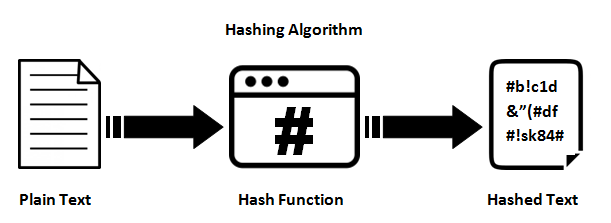
\includegraphics[width=0.75\textwidth]{img/bcrypt/Hashing.png}
    \caption{Representação de uma função de \emph{hash}.}
\end{figure}

Em geral, o \emph{hashing} é caraterizado como uma operação de sentido único, através da qual se gera um texto único sendo impossível de reverter para o texto original.
Embora esta noção esteja correta e seja impossível, através de um texto já processado por uma função de \emph{hash}, reconstruir o texto original em questão, este não é infalível.

\vspace{0.5cm}
\large{\textbf{Problema do \emph{hashing}}}


Embora o \emph{hashing} de passwords pareça uma solução segura, rapidamente foi descartado devido a ser extremamente suscetível a ataques baseado em \emph{rainbow tables}, também conhecidos por \emph{ataques de dicionário}.

A essência deste ataque não assenta no facto de calcular em tempo real \emph{hashes} aleatórios, mas sim utilizar valores de hash pré-calculados para toda e qualquer possível combinação de caracteres, utilizando para tal o método \emph{bruteforce}. 

Esta vulnerabilidade foi de tão larga escala que poderia quebrar \emph{99.9\%} de todas as combinações possíveis de 14 caracteres alfanuméricos em 11 minutos (utilizando a \emph{rainbow table} menos extensa, sendo que com tabelas mais extensas esta figura descia consideravelmente).

\cleardoublepage
\large{\textbf{A solução}}


A solução para este problema passou por diversificar ainda mais os \emph{hashes} gerados. Para tal foi adicionado um \emph{salt}, um dado aleatório adicionado ao input de uma dada função de \emph{hash} de modo a fazer qualquer password verdadeiramente única.

O método de autenticação ideal deve implementar ambos estes métodos, \emph{hashing} e \emph{salting}.

Um dos métodos mais comuns e seguros da atualidade, é o \emph{bcrypt}, uma implementação que recorre ao \emph{hashing} e \emph{salting}, tornando-a no perfeito candidato para utilização neste projeto.

\vspace{0.5cm}
\large{\textbf{Encriptação via \emph{bcrypt}}}
%TODO

\cleardoublepage

\begin{figure}[h]
    \centering
    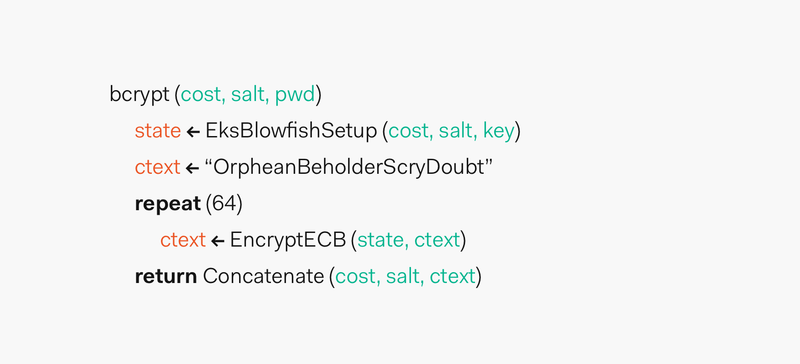
\includegraphics[width=1\textwidth]{img/bcrypt/bcrypt-algo.png}
    \caption{Pseudo código do algoritmo \emph{bcrypt}.}
\end{figure}

\subsection{Autenticação através do Auth.Gov}

\subsubsection{SSL}
\subsubsection{TLS}


\subsection{Autenticação de pedidos via API}
\subsubsection{JSON Web Token}


\subsection{Autenticação backend}